%%%
%
% $Autor: Wings $
% $Datum: 2021-05-14 $
% $Pfad: GitLab/MLEdgeComputer $
% $Dateiname: 
% $Version: 4620 $
%
% !TeX spellcheck = de_DE/GB
% !TeX program = pdflatex
% !BIB program = biber/bibtex
% !TeX encoding = utf8
%
%%%



\chapter{Project Magic Wand}

\section{Sources}




\begin{itemize}
    \item Hier findet man auch die librariy TensorFlow Lite: \URL{https://codelabs.developers.google.com/magicwand}
    \item \URL{https://github.com/tensorflow/tflite-micro-arduino-examples/tree/main}
    \item Auch interessant, aber nicht klar wozu:\URL{https://github.com/tensorflow/tflite-micro/}
    \item check this link: \URL{https://www.tensorflow.org/lite/microcontrollers}
\end{itemize}




\section{Introduction } 

Tiny Machine Learning (TinyML), is a rapidly growing subfield of applied ML. This area focuses on deploying simple yet powerful models on extremely low-power, low-cost microcontrollers at the network edge. TinyML models require relatively small amounts of data, and their training can employ simple procedures.

Furthermore, as TinyML can run on microcontroller development boards with extensive hardware abstraction, such as Arduino products, deploying an application onto hardware is easy. TinyML systems working in concert at the “edge” of the cloud-computing network.\cite{Reddi:2021}


This report discusses about Arduino and its environment and how we have implemented its functions in our project. Arduino is a development platform that can be used for easy integration of software and hardware. The boards by Arduino enables a user to read the input, and turn in to an output. The Arduino can be programmed according to the needs required by the user with a set of commands(Arduino Programming Langauge) using the Arduino \ac{ide}. \cite{Arduino:2021}
The report focusses on the hardware Arduino Nano BLE33 Sense which is a 3.3V AI enabled board. The Nano 33 BLE sense board is occupied three axis accelerometers. 

This implies that the sensor is able to detect the motion and inturn enables to calculate the acceleration produced in three directions. 
The objective of this report is to create a ``Magic Wand'' and implement the same into an Arduino Nano BLE33 sense  board. Gestures namely ``wing'', ``ring'' and ``slope'' will be recognised by the board when the wand is waved. The direction of motion for the recognition of the gestures are shown in the figure \ref{gestures}.

\begin{figure}
    
    \begin{center} 
        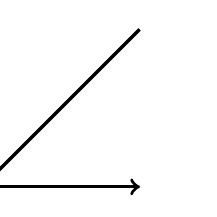
\begin{tikzpicture}
            % define point
            \hspace{-0.6cm}
            \coordinate (A)  at (2, 2);
            \coordinate (O)  at (0, 0);
            \coordinate (B)  at (2, 0);
            % angle  
            \draw[thick] (A) -- (O) -- (B);
            %\draw pic[draw=black,angle radius=20,angle eccentricity=1.4]
            %{angle = B--O--A};
            %\pic [draw,"$\alpha_1$",angle radius=20,->,angle eccentricity=1.4]
            %  {angle = B--O--A};
            \draw [->, very thick] (2,2) -- (0,0)  node [midway, above] {\scriptsize };
            \draw [->, very thick] (0,0) -- (2,0)  node [midway, above] {\scriptsize };
        \end{tikzpicture}
        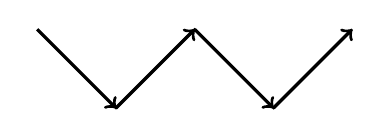
\begin{tikzpicture}
            \hspace{0.1cm}
            % define point
            \coordinate (A)  at (1, 1);
            \coordinate (O)  at (2, 0);
            \coordinate (B)  at (3, 1);
            \coordinate (C)  at  (4,0);
            \coordinate (D) at  (5,1);
            % angle  
            \draw[thick] (A) -- (O) -- (B) -- (C)-- (D);
            %	\draw pic[draw=black,eccentricity=2.9]
            %\pic [draw,"$\alpha_1$",angle radius=20,->,angle eccentricity=1.4]
            %  {angle = B--O--A};
            \draw [->, very thick] (1,1) -- (2,0)  node [midway, above] {\scriptsize };
            \draw [->, very thick] (2,0) -- (3,1)  node [midway, above] {\scriptsize };
            \draw [->, very thick] (3,1) -- (4,0)  node [midway, above] {\scriptsize };
            \draw [->, very thick] (4,0) -- (5,1)  node [midway, above] {\scriptsize };
        \end{tikzpicture}
        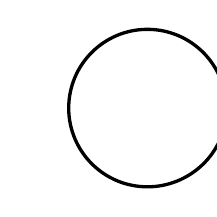
\begin{tikzpicture}
            \hspace{0.5cm}
            \draw[->,very thick] (0,0) arc[radius=1cm,start angle=0,delta angle=359];
        \end{tikzpicture}
        \caption{\textbf{Gestures used namely Slope, W and ring}} \label{gestures} 
    \end{center} 
\end{figure} 
The Arduino can also be programmed such that the \ac{led}  the hardware blinks according to the commands given in relation to the gestures waved by the hand. For example , the Arduino can be programmed to indicate a green light when a ``wing'' is waved , red for ``slope'' and  blue for ``ring''.

When the wand is moved in the direction as shown in the figure, the gesture interpreted by the board is transformed into a visual output. 

To construct magic wand, attach the Arduino Nano BLE 33 sense board to the end of a stick. Then feed the accelerometer’s output into a deep learning model, which will perform classification to tell whether a known gesture was made. \cite{Warden:2020}


Gestures collected using the built-in multi-dimensional sensor on the Arduino board are able to understand the complex data and the model can be trained such that it understands the complex data and embeds them in to a microcontroller that is Arduino Nano 33 BLE Sense. Specifically, it uses TensorFlow Lite to run Convolutional Neural Network model to recognize gestures with an accelerometer.  If you’re successful casting the spells, you will see the corresponding gesture as a visual output on the screen and the Arduino board should be lit according to the command given by the user.



Heuristic function is used for this application, which is a function that expresses the knowledge of gestures as a function in code. To create a heuristic we need domain knowledge, programming and mathematical expertise. A heuristic algorithm expresses human knowledge and understanding. The data obtained from the accelerator is mathematically converted to get a desired output or the gestures which we want to cast. 

Instead of designing a heuristic algorithm from scratch, a machine learning developer can find a suitable model architecture, collect and label a dataset, and iteratively create a model through training and evaluation. \cite{Warden:2020}


There is no pre-processing done in the model, instead the accelerometer values are directly taken as input. Then it runs inference and then processes the output. The gestures trained are wing (w), ring (o) and  slope ($\angle$) and if the input is recognized as valid, it prints a visual output of the gestures on the terminal and it reacts to each spell by lighting an LED. In case any of the gestures are not recognised, there will also be an output to notify that the gesture is "unknown".


From the initial planning phase, various challenges encountered are:-

\begin{itemize}
    \item Creating a dataset on the 4 gestures , especially unknown gesture as the amount of data to be recorded for the unknown gesture has no limit and would require a concrete database.
    
    \item Gesture should have a minimum wave time of 5 seconds, else it may give false readings.
    
    \item Gestures waved should not be of a very long time duration which might make the accelerometer to record false reading giving a false output.
    
    \item Programming the Arduino Nano.
    
    \item Interference on cheap or low power hardware.
    
    \item Incorporating Arduino and the Magic Wand.
    
    
\end{itemize}
\bigskip
Most of the challenges faced were addressed with knowledge imparted from the book TinyML. For programming the Arduino, the Arduino guide was referred to and the application required was downloaded from the Arduino website. 

The report initially talks about the Domain Knowledge acquired for - Magic Wand- Arduino Nano BLE33 Sense and other components involved in the project, special emphasis is given to IMU sensors (LSM9DS1). The involvement of \ac{cnn} in the project is discussed in the next section followed by the application of \ac{kdd} processes. The \ac{kdd} section discusses about the steps involved in creating a target dataset, selection, preparation and transformation of the dataset followed by data mining which discusses about the patterns found in the database. 

The report further talks about the implementation and deployment of the known results obtained from the initial phase, it then concludes with the future scope and the improvements that can be incorporated in the future.




\section{Development}

This section talks about how the KDD process is implemented and the steps followed for each of the KDD Processes starting with the preparation of Databases

\subsection{Database}

Since there are no existing databases for the model a new database will be created. The database is a .txt file which contains raw data from the accelerometer  readings recognized by the Arduino Nano 33 BLE Sense. Since the way how the gesture is recorded by a person varies from one to another, gestures of three people are recorded as we are a group of three members. In order for the database to have a vast amount of data, each person will record a minimum of 50 trials for each gesture. In order for the database to be more accurate data from both ahnds of the three users were used. This would improve the efficiency and  effectiveness of the database making it more concrete. There is also a possibility to add further data into our model which would improve our model over time.The size of the database thus created will be very small that would be less than 2 MB.Obtaining sufficient data is one of the major concerns in a machine learning project and the amount of data involved in our data set is very small. The data thus created will be further used in the next step ``Data Preparation and Transformation'' where this raw data is further processed and the outliers are identified and removed if necessary. \cite{Warden:2020}

\subsection{Data Preparation}

%%%%%%%%%%%%%%%%%%%%%%%%%%%%%%%
This section discusses about how to shape our data and how we can use it for training. Three gestures are to be recognized by our machine learning model namely wing, slope and ring. Since we are not intending to use any existing databases,  in order to prepare the data we will give multiple inputs for a single gesture and save it as model data for the gesture. When a gesture for example - ``wing'' is waved using the wand, the acceloremeter present in the microcontroller detects the movement by using the coordinates in x,y and z axes. The same process is repeated multiple number of times for the dataset to be as large as possible. The advantage of creating a database with more inputs allows the machine learning model to be more accurate and provide better and efficient results. The same process is repeated for the remaining gestures namely ring, slope and unknown.
With the data available for the above gestures, we can use it to train a model. The data that is available is split in to two namely as training data and test data.

The major challenge while preparing data can be the presence of outliers or anomalies where there are unexpected values. This can be overcome by feeding our model with more data so that the model is efficient. \cite{Warden:2020}

The different steps involved in preparing data can be as follows according to \cite{Warden:2020}

\begin{description}
    \item[Understanding the problem] The problem, which in our case is collection of data consisting of gestures. The main problem is sub divided in to many parts for easy preparation of data.
    \item[Preparation of data] The step deals with converting the raw data in to machine learning language that can be interpreted by the compiler. 
    \item[Evaluation of data] This step deals with evaluating the model after collection of the nexessary data. This data is then checked for its correctness and analysis is done according to the accuracy of output obtained. 
    \item[Finalizing the data] The model is tested with various parameters and the data is validated. If the results obtained are according to our requirements, the resulting dataset is finalized.
\end{description}

The same steps are repeated for various gestures and the final database is created.

\subsubsection{Preparation of Datasets for the Magic Wand}

Since the amount of data required for creation of a database is very small the database will be prepared by us. The first set of data that we are trying to capture the movement is for the gesture ``W''. The steps involved in capturing a W is mentioned below. \cite{Warden:2020}
\vspace{5mm}
\begin{center}
    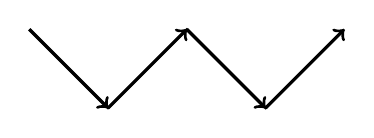
\begin{tikzpicture}
        % define point
        \coordinate (A)  at (1, 1);
        \coordinate (O)  at (2, 0);
        \coordinate (B)  at (3, 1);
        \coordinate (C)  at  (4,0);
        \coordinate (D) at  (5,1);
        % angle  
        \draw[thick] (A) -- (O) -- (B) -- (C)-- (D);
        %	\draw pic[draw=black,eccentricity=2.9]
        %\pic [draw,"$\alpha_1$",angle radius=20,->,angle eccentricity=1.4]
        %  {angle = B--O--A};
        \draw [->, very thick] (1,1) -- (2,0)  node [midway, above] {\scriptsize };
        \draw [->, very thick] (2,0) -- (3,1)  node [midway, above] {\scriptsize };
        \draw [->, very thick] (3,1) -- (4,0)  node [midway, above] {\scriptsize };
        \draw [->, very thick] (4,0) -- (5,1)  node [midway, above] {\scriptsize };
    \end{tikzpicture}
    \captionof{figure}{\textbf{Wing Gesture \cite{Warden:2020}}}
\end{center}
\begin{itemize}
    \item The device is first moved down and to the right.
    \item Then the device is moved up and to the right.
    \item The device is then moved down and to the right.
    \item  The device is then moved up and to the right again. 
    
\end{itemize}

Shows a sample of real data captured during the ``wing'' gesture, measured in milli-Gs.  

The process involved in capturing a ring are as follows. \cite{Warden:2020}


\begin{center}
    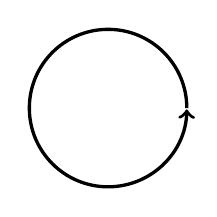
\begin{tikzpicture}
        \draw[->,very thick] (0,0) arc[radius=1cm,start angle=0,delta angle=359];
    \end{tikzpicture}
    \captionof{figure}{\textbf{Ring Gesture \cite{Warden:2020}}}
\end{center}

\begin{itemize}
    \item Trace a clockwise circle using the wand.
    
    \item Aim again to take around a second to perform gesture.
    
\end{itemize}



The steps involved in waving the slope gesture is mentioned below \cite{Warden:2020}:

\begin{center}
    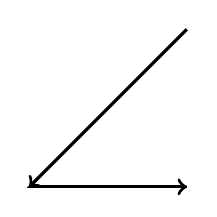
\begin{tikzpicture}
        % define point
        \coordinate (A)  at (2, 2);
        \coordinate (O)  at (0, 0);
        \coordinate (B)  at (2, 0);
        % angle  
        \draw[thick] (A) -- (O) -- (B);
        %\draw pic[draw=black,angle radius=20,angle eccentricity=1.4]
        %{angle = B--O--A};
        %\pic [draw,"$\alpha_1$",angle radius=20,->,angle eccentricity=1.4]
        %  {angle = B--O--A};
        \draw [->, very thick] (2,2) -- (0,0)  node [midway, above] {\scriptsize };
        \draw [->, very thick] (0,0) -- (2,0)  node [midway, above] {\scriptsize };
    \end{tikzpicture}
    \captionof{figure}{\textbf{Slope Gesture \cite{Warden:2020}}}
\end{center}

\begin{itemize}
    \item The device is first moved down and to the left.
    \item Then the device is moved to the right.
    \item Finally you should get a corner of the triangle as shown in the figure.
\end{itemize}



The process is repeated until around 15 readings are captured by the wand for Data Preparation and Transformation. 

In order to consider the unknown readings, we will be carrying out an other set of procedures to feed with unknown data. This would help the wand recognize any unknown gesture and gives the output stating that it is false. \cite{Warden:2020}




All readings that are recorded in a unique text file for each gesture. The files \FILE{.txt} contains raw accelerometer data that would later be transformed in to machine learning language that should be interpreted by the compiler. \cite{Warden:2020}







\subsection{Data Transformation \& Mining}
%%%%%%%%%%%%%%%%%%%%%%%%%
It is in the data mining step that the model is actually built, However before we start the process the algorithm that needs to be used has to be decided. As discussed in the previous section, the dataset is divided equally so that model testing and evaluation is also done to re-confirm the model works fine.

We need to run a simple program to log accelerometer data to the serial port when the gestures are being performed. \cite{Warden:2020}


All the codes used from Github are re-edited to suit the dataset.

\subsubsection{Training the Model}

To get started we need to modify one of the examples in  SparkFun Edge Board Support Package (BSP) such that we can input the data set that we captured.First, follow SparkFun's ``Using SparkFun Edge Board with Ambiq Apollo3 SDK'' guide to set up the Ambiq SDK and SparkFun Edge BSP. Then the code needs to be changed.\cite{Warden:2020}

The program will then be ready to take the dataset as the input. We then need to build the example application and flash it to the device.

The next step is to capture the required data, as mentioned in the previous section, the 3 members of the group will perform the required gestures and create the dataset. For that, we need to open the terminal window and run the following command:

\medskip

\SHELL{script output.txt}

\medskip

In the next screen connect to device \textcolor{blue}{``115200''}. Post the measurements from the accelorometer will show up on the screen. The values will also be saved to a file \FILE{output.txt}. \cite{Warden:2020}

\begin{figure}
    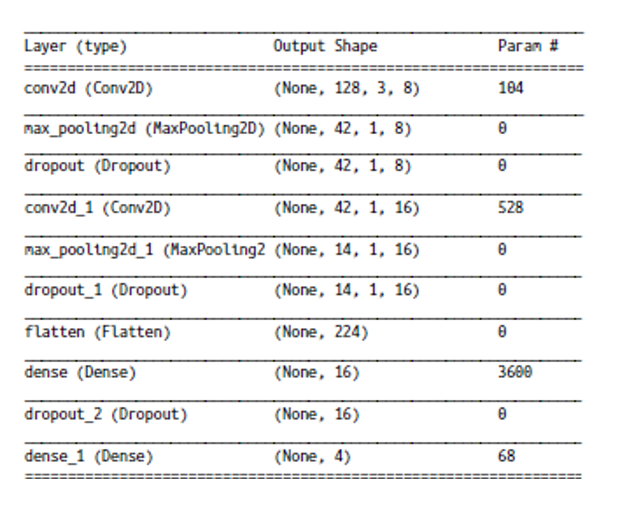
\includegraphics[width=\linewidth]{Nano33BLESense/337.png}
    \caption{\textbf{\ac{cnn} sequence to classify gestures. Source : \cite{Warden:2020}}}
    \label{fig:T1}
\end{figure}

\bigskip 

The text file will contain the data in accordance how it is required by the training set. In order to get a good quality dataset, the same gestures are repeated again as much as possible and then the program is exited. Then the next group member makes the similar file  \FILE{output.txt}. We need to press the button marked 14 to stop logging the acceleration data. \cite{Warden:2020}

We need to rename the folders for files \FILE{output.txt} as per the names of the person who performed the gestures, this helps to differentiate the datasets for testing and validation purposes. \cite{Warden:2020}  

Data for unknown category also is then added, so that when a different gesture is shown, the model identifies it as an unknown gesture.  The folowing are the steps for training the model:

\begin{itemize}
    \item Loading the tensor board.
    \item Codes are run to begin the training on Google Colab.
    \item The file \FILE{data\_augmentation} is run to train the model better as it has changed values of acceleration as will it give the model more input values.
    \item We will then start to see output values appearing on the screen (These are the memory size of the model)
\end{itemize}

The training then ramps up and the validation accuracy gets better with time.





%%%%%%%%%%%%%%%%%%%%%%%%%%%%
%\subsection{Model/Patterns}
%%%%%%%%%%%%%%%%%%%%%%%%%%%%




%%%%%%%%%%%%%%%%%%%%%%%%%%%%%%%%%%


\subsection{Model}

In  model for this project,  we transform a sequence of 128 three-axis accelerometer readings, representing
around five seconds of time, into an array of four probabilities: one for each gesture,
and one for ``unknown''.  
\ac{cnn}s are used when the relationships between adjacent values contain important information\cite{Warden:2020}. 
A \ac{cnn} with numerous layers may learn to recognize each gesture by analyzing its component parts. For example, a network might learn to recognize up-and-down motions and that combining two of them with the appropriate z- and y-axis movements results in a "wing" gesture\cite{Warden:2020}.
A \ac{cnn} accomplishes this by learning a series of filters organized in layers. Each filter learns to recognize a specific type of data feature. When it identifies this feature, it sends this high-level data to the network's next tier. One filter in the network's first layer, for example, might learn to recognize something as simple as a period of upward acceleration. When it identifies such a structure, it passes this information to the next layer of the network.\cite{Warden:2020}
The outputs of earlier, simpler filters are mixed together to build larger structures in subsequent layers of filters. For example, the "W" shape in the "wing" gesture could be represented by a series of four alternating upward and downward accelerations.
The noisy input data is gradually turned into a high-level, symbolic representation in this process. Network's subsequent layers can use this symbolic representation to figure out which gesture was made. \cite{Warden:2020}

For data acquisition we are using \ac{imu} signals \ref{fig:IMU}. IMU is the electronic component which contains the accelerometer. The object \ac{imu} comes from the Arduino  library LSM9DS1.\index{LSM9DS1}

\begin{figure}[h!]
    \begin{center}
        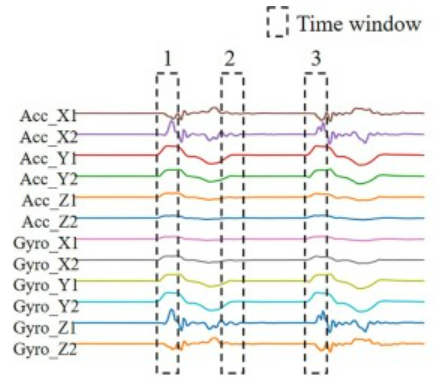
\includegraphics[width=100mm]{Nano33BLESense/IMU.png}
        \caption{\textbf{\ac{imu} signals \cite{Xu:2022} }}
        \label{fig:IMU}
    \end{center}
\end{figure}

Convolutional layer directly receives network's input, which is a sequence of raw accelerometer data. The input's shape is provided in the input shape argument. It's set to \PYTHON{(seqlength, 3, 1)}, where seqlength is the total number of accelerometer measurements that are passed (\PYTHON{128}\ by default). Each measurement is composed of three values, representing the x, y, and z-axes. \cite{Warden:2020}

\begin{figure}[h!]
    \begin{center}
        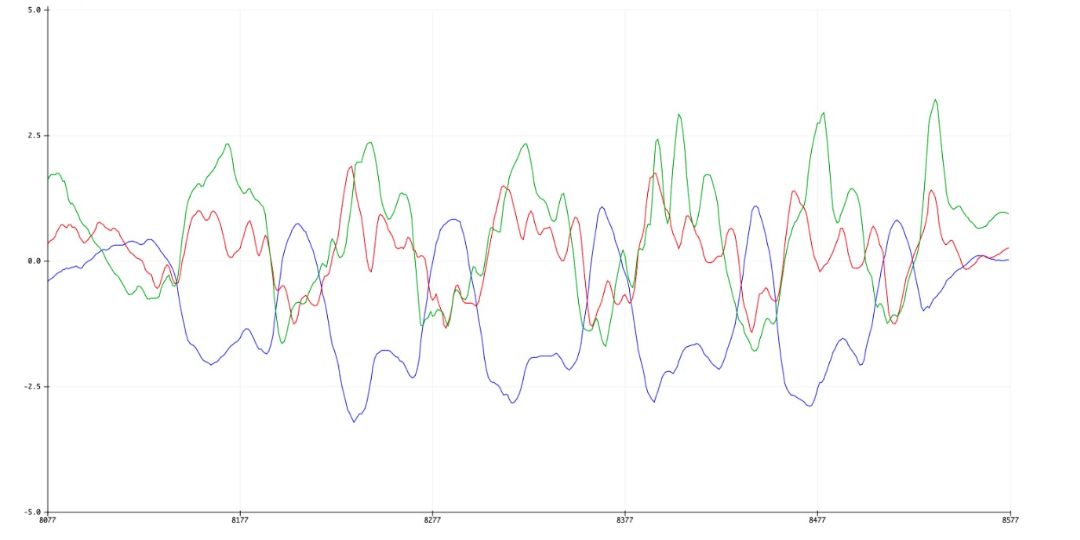
\includegraphics[width=100mm]{Nano33BLESense/IMUAccelero.png}
        \caption{\textbf{\ac{imu} Accelerometer Graph \cite{Warden:2020}}}
        \label{fig:IMU}
    \end{center}
\end{figure}

The job of the convolutional layer is to take this raw data and extract some basic features
that can be interpreted by subsequent layers. The arguments to the function \PYTHON{Conv2D()} determine how many features will be extracted.

The function \PYTHON{Conv2D()} is where we provide the dimensions of this window. In this case, it's \PYTHON{(4, 3)}.
This means that the features for which our filters are hunting span four consecutive
accelerometer measurements and all three axes. Because the window spans four
measurements, each filter analyses a small snapshot of time, meaning it can generate
features that represent a change in acceleration over time. You can see how this works
in \ref{fig:129} \cite{Warden:2020}

\begin{figure}[h!]
    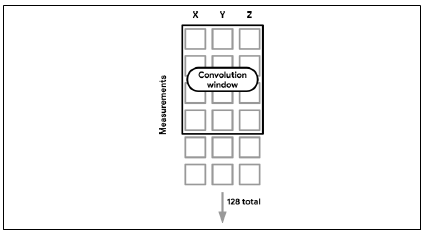
\includegraphics[width=\linewidth]{Nano33BLESense/129.png}
    \caption{\textbf{A convolution window overlaid on the data. \cite{Warden:2020}}}
    \label{fig:129}
\end{figure}

The padding argument determines how the window will be moved across the data.
When padding is set to "same", the layer's output will have the same length (128) and
width (3) as the input. Because every movement of the filter window results in a single
output value, the "same" argument means the window must be moved three times
across the data, and 128 times down it. As soon as the convolution window has moved across all the data, using each filter to create eight different feature maps, the output will be passed to our next layer, MaxPool2D.
This MaxPool2D layer takes the output of the previous layer, a (128, 3, 8) tensor,
and shrinks it down to a (42, 1, 8) tensor a third of its original size. It does this by
looking at a window of input data and then selecting the largest value in the window
and propagating only that value to the output. The process is then repeated with the
next window of data. The argument provided to the MaxPool2D function, (3, 3),
specifies that a 3 × 3 window should be used. By default, the window is always moved
so that it contains entirely new data. \ref{fig:1212} shows how this process works. \cite{Warden:2020}

\begin{figure}[h!]
    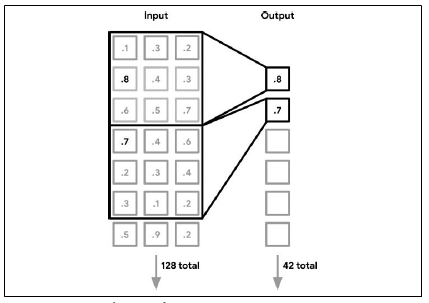
\includegraphics[width=\linewidth]{Nano33BLESense/1212.png}
    \caption{\textbf{Max Pooling. \cite{Warden:2020}}}
    \label{fig:1212}
\end{figure}

The goal of a \ac{cnn} is to transform a big, complex input tensor into a small, simple output.
The MaxPool2D layer helps make this happen. It boils down the output of our first
convolutional layer into a concentrated, high-level representation of the relevant
information that it contains.
By concentrating the information, we begin to strip out things that aren't relevant to
the task of identifying which gesture was contained within the input. Only the most
significant features, which were maximally represented in the first convolutional
layer's output, are preserved.
After we've shrunk the data down, it goes through a Dropout layer. Dropout is a regularization technique; regularization is the process of improving machine learning models so that they are less likely to overfit their training data. Dropout is a simple but effective way to limit overfitting.
By randomly removing some data between one layer and the next, we force the neural
network to learn how to cope with unexpected noise and variation. Adding dropout
between layers is a common and effective practice. The dropout layer is only active during training. During inference, it has no effect; all of the data is allowed through. \cite{Warden:2020}

This continues the process of distilling the original input down to a smaller, more
manageable representation. The output, with a shape of (14, 1, 16), is a multidimensional
tensor that symbolically represents only the most significant structures
contained within the input data.

If we want to, we can continue the process of convolution and pooling. The
number of layers in a \ac{cnn} is just another hyperparameter that we can tune during model development. However, during the development of this model, we found that two convolutional layers was sufficient.\ref{fig:CNN2} shows the sequence.

\begin{figure}[h!]
    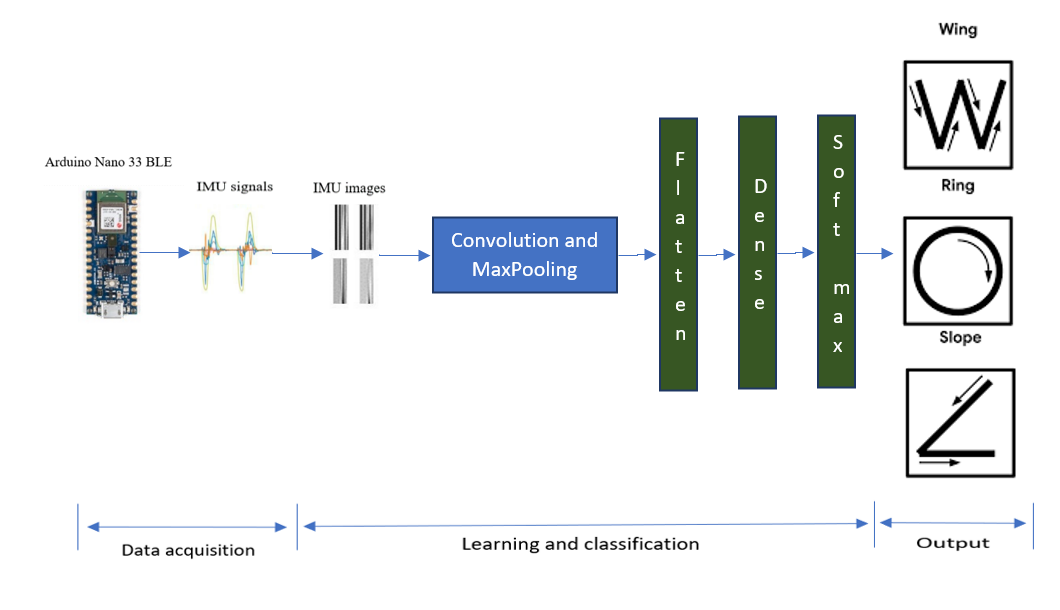
\includegraphics[width=\linewidth]{Nano33BLESense/CNN2.png}
    \caption{\textbf{\ac{cnn} sequence to classify Wing,Ring and Slope.}}
    \label{fig:CNN2}
\end{figure}

We flatten the data and feed it into a Dense layer (also known as a fully connected layer) to find out the major features within our input. 
The Flatten layer is used to transform a multidimensional tensor into one with a
single dimension. In this case, our (14, 1, 16) tensor is squished down into a single
dimension with shape (224).
``It's then fed into a Dense layer with 16 neurons. This is one of the most basic tools in
the deep learning toolbox: a layer where every input is connected to every neuron. By
considering all of the data, all at once, this layer can learn the meanings of various
combinations of inputs. The output of this Dense layer will be a set of 16 values representing
the content of the original input in a highly compressed form''.\cite{Warden:2020}
Our final task is to shrink these 16 values down into 4 classes
This layer has four neurons; one representing each class of gesture. Each of them is
connected to all 16 of the outputs from the previous layer. During training, each neuron
will learn the combination of previous-layer activations that correspond to the
gesture it represents.
The layer is configured with a "softmax" activation function, which results in the layer's
output being a set of probabilities that sum to 1. This output is what we see in the
model's output tensor.
"This type of model architecture—a combination of convolutional and fully connected
layers—is very useful in classifying time-series sensor data like the measurements we
obtain from our accelerometer. The model learns to identify the high-level features
that represent the “gesture” of a particular class of input".\cite{Warden:2020}

Once we have a result from all the inferences in the model, inorder to ensure there is no false positive the model's output tensor is given as input to a function called PredictGesture().

Two main actions are carried out by this function. It checks whether the getsures probability meets a minimum threshold and also checks if the gesture has been detected over a certain number of inferences. 

The minimum number of inferences to confirm a gesture varies from the type of gesture as different gestures take different times to perform. The number of inferences required for each gesture is located in the file constants.cc. \cite{Warden:2020}

This function returns the predicted gesture by returning numeric values 0,1, 2,3 for Wing, Ring, Slope and unknown respectively. 
Initially the "prediction scores" obtained from the main is passed on to the function in which a ``maxPredictionScore'' and ``maxPrediction Index''.
These values  above are then compared "kNoGesture" and "kDetectionThrehsold" and then a value of found gesture variable is found which is equal to max predicition index. This value is then returned to the main function and passed to output\_handler() which then displays the recognised gesture. \cite{Warden:2020}


%\subsection{Using the Model in Arduino Nano 33 BLE Sense}
%
%Once the model is ready to be deployed, we need to copy the model's data as formatted by xxd -i, into \textcolor{red}{magic\_wand\_model\_data.cc}. This is to deploy the model to the Arduino.
% 
% We then need to update the values in the accelerometer\_handeler.cc depending upon the time taken for performing the gestures by the group member.
% Once that is updated, we then update the final code and the code is flashed to the device.\cite{Warden:2020}

\subsection{Evaluation and Verification}

Once we get the model ready, it is important to test the model with a different dataset. This helps us confirm our model will work fine with gestures from other persons as well. To test the model we need to now call the Keras's \textcolor{red}{model.evaluate()} function.\cite{Warden:2020}



We can also use a confusion matrix to check the performance of the model. An example of a confusion matrix according to the \cite{Warden:2020} is shown in \ref{fig:CFM} which is calculated by \textcolor{red}{ tf.math.confusion$\_$matrix()} function:

\begin{figure}[h!]
    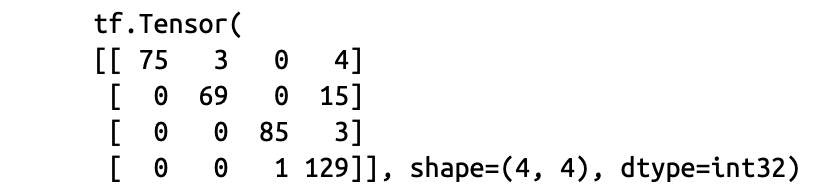
\includegraphics[width=\linewidth]{Nano33BLESense/CFM.png}
    \caption{\textbf{ Sample Confusion Matrix for the dataset \cite{Warden:2020}}}
    \label{fig:CFM}
\end{figure}



The confusion matrix fuction tells us how much the predicted class of each input in the test dataset agrees to the actual value. It basically tells us the weak points of our model. We can then prepare the dataset again knowing the weak points and train the model once again.\cite{Warden:2020} which improves our model over time



%\subsection{Developers Manual}

%This developers manual is a module developed for understanding the working and functioning of an Arduino Nano BLE 33 Sense which was used in creating a magic wand.
%The hardware and softwares used with explanations on the functioning of the code is mentioned. The various classess and functioned defined in the main program are also mentioned which would help a developer to develop the project to a further stage at later point on time.





\section{Deployment}

In the above sections, the complete details with regards to implementing the project is discussed. In the deployment phase the knowledge acquired in the development phase is applied and implemented. 

%By performing all the steps of Knowledge Discovery Database (KDD) process, machine learning model is ready to use or deploy on any computer. The trained model is very usefull for embedded device for making the edge computing application. The one  we can deploy the model on small edge devices like Arduino Nano 33 BLE Sense and use in Internet of things (IOT), and Artificial Intelligence (AI) application. Before deploying we need to make sure that, the trained model has properly evaluate and verify for unseen data or not, either the model is able to predict and evaluate the unseen situation, as the human want. It depends upon the usage and type of model we train, either it could be supported low processing devices or not.
%\\
%
%KDD focuses on the overall process of knowledge discovery from data, including how the data are stored and accessed, how algorithms can be scaled to massive data sets ultimate and still run efficiently, how results can be interpreted and visualized, and how the overall man-machine interaction can usefully be modeled and supported.\href{https://bit.ly/2YzOxis}{KDD}

%Model in use.
\subsection{Software}

\subsection{Precondition}

TensorFlow Lite for Arduino, see \ref{chap:TensorFlowLiteArduino}, is used. Additionally the library for the IMU, see \ref{chap:InertialMeasurementUnit}, must be installed.

\Mynote{How to check}


\Mynote{cite \URL{https://codelabs.developers.google.com/magicwand}}

\begin{itemize}
  \item Hier findet man auch die librariy TensorFlow Lite: \URL{https://codelabs.developers.google.com/magicwand}
  \item \URL{https://github.com/tensorflow/tflite-micro-arduino-examples/tree/main}
  \item Auch interessant, aber nicht klar wozu:\URL{https://github.com/tensorflow/tflite-micro/}
  \item check this link: \URL{https://www.tensorflow.org/lite/microcontrollers}
\end{itemize}



\subsubsection{Recognizing Gestures}

This code snippet in \ref{fig:img13} recognizes gestures. The program initially checks if the wand moves and then a signal is given to the compiler for recording the gestures. A switch case statement checks whether the wand stays still or the wand keeps moving.

\begin{figure}[h!]
    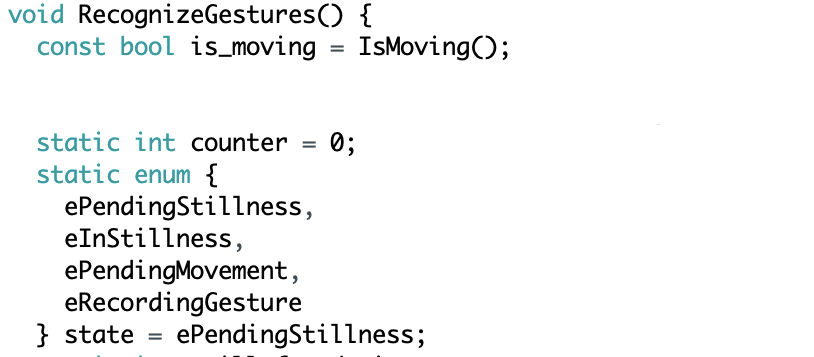
\includegraphics[width=\linewidth]{Nano33BLESense/RecognizeGesture.png}
    \caption{\textbf{Function to Recognize gestures}}
    \label{fig:img13}
\end{figure}

\subsubsection{Prediction of Gestures}

\begin{figure}[h!]
    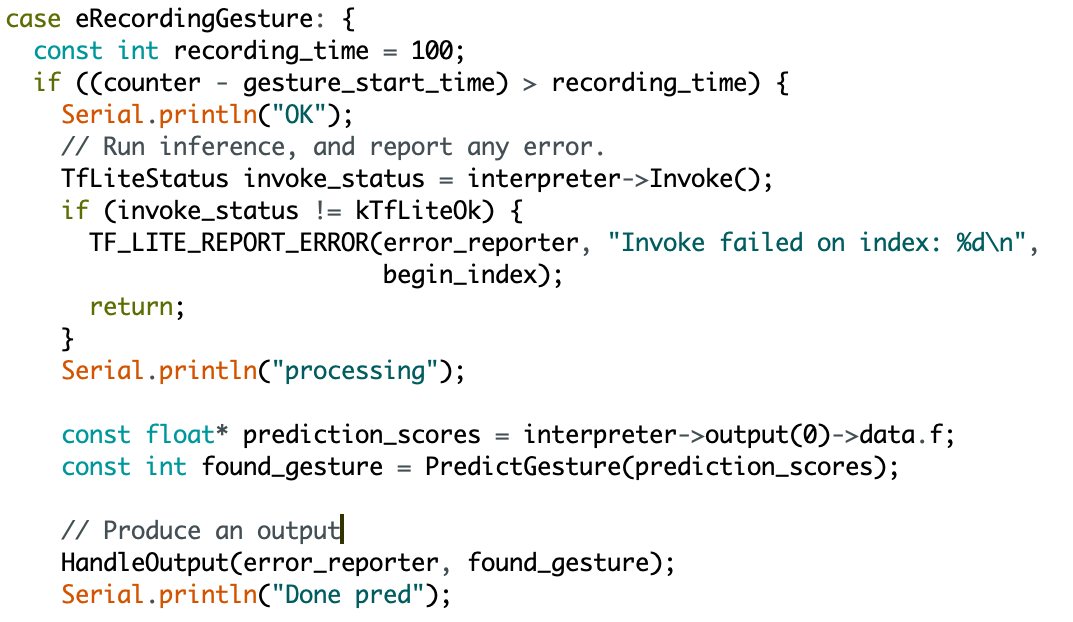
\includegraphics[width=\linewidth]{Nano33BLESense/RecordingGesture.png}
    \caption{\textbf{Code snippet that shows processing of the waved gestures}}
    \label{fig:img14}
\end{figure}

The code snippet in \ref{fig:img14} how a gesture is being recorded is shown in this code snippet. The gesture waved is passed to a function PredictGesture() and the value is stored in to a variable. Which is then passed to the function HandleOutput() to display the gesture waved. The session ends by displaying "Done prediction" and the hardware waits for the new gesture to be fed.

\subsubsection{Pending Movement}
The code in \ref{fig:img9} checks for any pending movement and waits for a new gesture to be recorded.
\begin{figure}[h!]
    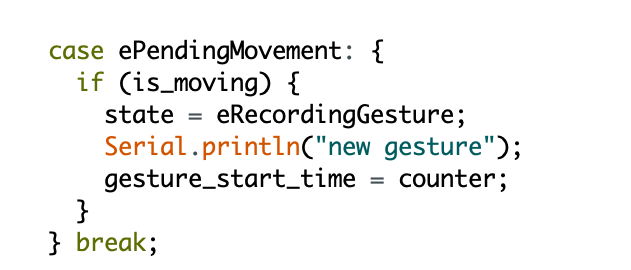
\includegraphics[width=\linewidth]{Nano33BLESense/img9.png}
    \caption{\textbf{Switch case statement, Pending Movement}}
    \label{fig:img9}
\end{figure}

\subsubsection{Training or Recognizing} 
The code in \ref{fig:img10} snippet has a boolean expression at the end for which if the value is "false" the code works like the data to be captured. Change the expression in to "true" to start training the model and gather the values.

\begin{figure}[h!]
    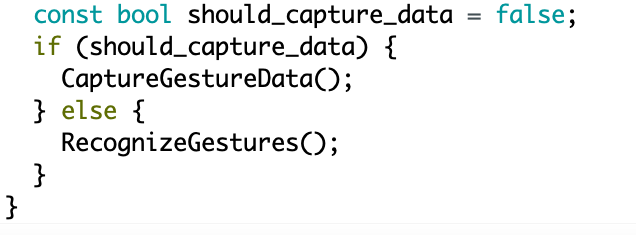
\includegraphics[width=\linewidth]{Nano33BLESense/constbool.png}
    \caption{\textbf{Code snippet that explains to train or to capture gestures}}
    \label{fig:img10}
\end{figure}


\subsubsection{Printing the output}


\begin{figure}[h!]
    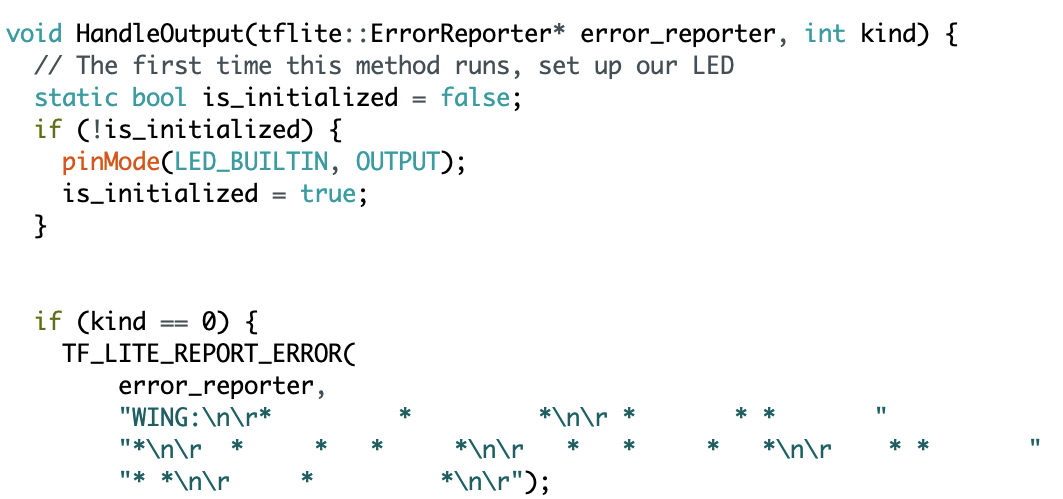
\includegraphics[width=\linewidth]{Nano33BLESense/HandleOutput.png}
    \caption{\textbf{Code snippet displaying a Wing gesture}}
    \label{fig:img12}
\end{figure}

The code snippet in \ref{fig:img12} shows how the output is being printed using "*" using different line spacing methods. An example of how the wing gesture is being displayed is shown in the figure.

\subsubsection{Prediction Score}
The code snippet in \ref{fig:img11}  allows the user to tweak the threshold values of various gestures. A higher value of kDetectionThreshold gives more robust values. But if the results achieved are not very good, more training has to be carried out.
\begin{figure}[h!]
    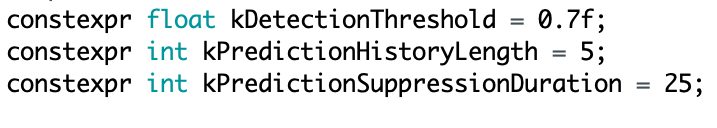
\includegraphics[width=\linewidth]{Nano33BLESense/constexpr.png}
    \caption{\textbf{The value of constants and constant thresholds in the program}}
    \label{fig:img11}
\end{figure}

\subsubsection{ASCII outputs for Wing, Ring , Slope and Unknown}

This code snippets show the various outputs displayed for \ref{wing} for Wing, \ref{slope} for Slope, \ref{ring} and for unknown \ref{unknown} 
\begin{figure}[h!]
    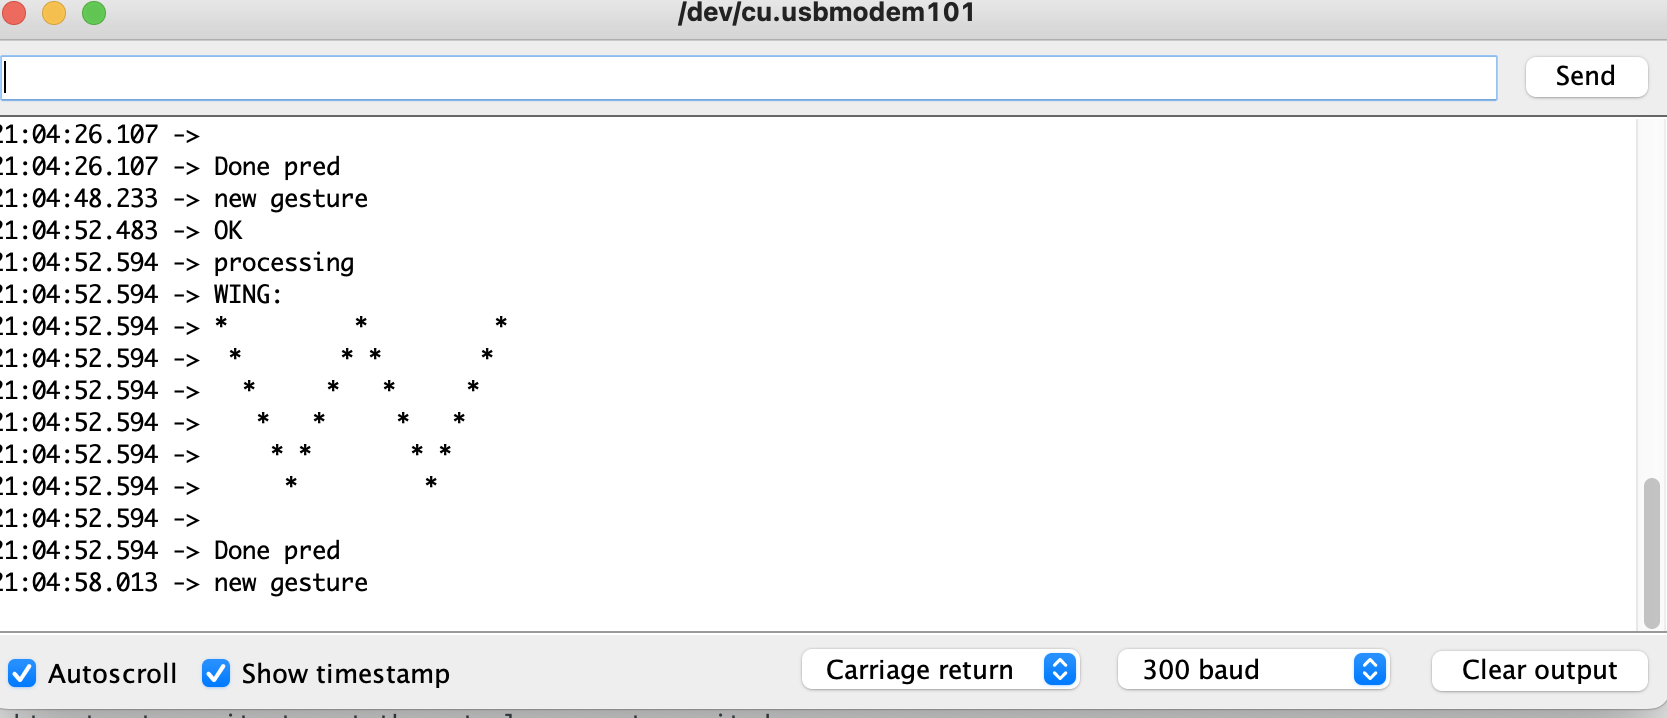
\includegraphics[width=\linewidth]{Nano33BLESense/Wing.png}
    \caption{\textbf{The displayed Wing gesture}}
    \label{wing}
\end{figure}

\begin{figure}[h!]
    \includegraphics[width=\linewidth]{Nano33BLESense/slope.png}
    \caption{\textbf{The displayed slope gesture}}
    \label{slope}
\end{figure}

\begin{figure}[h!]
    \includegraphics[width=\linewidth]{Nano33BLESense/ring.png}
    \caption{\textbf{The displayed ring gesture}}
    \label{ring}
\end{figure}

\begin{figure}[h!]
    \includegraphics[width=\linewidth]{Nano33BLESense/unknown.png}
    \caption{\textbf{The unknown gesture}}
    \label{unknown}
\end{figure}










\bigskip
\newpage







\subsection{Program Flow Code}

On clicking the option "Manage Libraries" a new window shows up where a person can search for the libraries and install them.

\chapter{Magic Wand Program Workflow}



\tikzstyle{decision} = [diamond, draw, fill=white, 
text width=5.5em, text badly centered, node distance=3cm, inner sep=0pt]
\tikzstyle{block} = [rectangle, draw, fill=blue!20, 
text width=9em, text centered, rounded corners, minimum height=2.5em]
\tikzstyle{line} = [draw, -latex']
\tikzstyle{cloud} = [draw, ellipse,fill=white, node distance=2cm,
minimum height=2em]
\begin{center}
    \begin{tikzpicture}[node distance = 2.2cm, auto]
        
        \node [cloud,fill=green!50,node distance=1cm] (init) {Start};
        \node [block, below of=init] (start) {Waiting for movement};
        \node [decision,fill=yellow!20,below of=start] (select) {Check if moving};
        \node [block, left of=select,node distance=5cm] (invalid){Wand is still in stillness};
        %		\node [block, below of=select,node distance=3cm] (neighbour) {Pending movement};
        \node [block, below of=select, node distance=3cm] (distance) {Record gesture};
        \node [block, below of=distance,node distance=2cm] (update) {Gesture Predictor};
        \node [block, below of=update,node distance=2cm] (run) {Check the predicted score};
        \node [decision,fill=yellow!20,below of=run, node distance=3cm] (decide) {Gesture found?};
        \node [cloud,fill=red!50, left of=decide,node distance=5cm] (none){"Unkown"};
        \node [block, below of=decide, node distance=3cm] (stop) {Display Output};
        \node [cloud,fill=red!50, below of=stop,node distance=2cm] (end) {End};
        \path [line] (init) -- (start);
        \path [line] (start) -- (select);
        \path [line] (select) --node {Yes} (distance);
        \path [line] (select) -- node[near start]{No}  (invalid);
        \path [line] (invalid) |-  (start);
        %	\path [line] (neighbour) -- (distance);
        \path [line] (distance) -- (update);
        \path [line] (update) -- (run);
        \path [line] (run) -- (decide);
        \path [line] (decide) -- node {Yes}(stop);
        \path [line] (decide) -- node[near start]{No}  (none);
        \path [line] (stop) -- (end);
        %	\path [line] (solution) -- (stop);
        
    \end{tikzpicture}
\end{center}


The flow chart depicts a basic flow of the program. Initially the wand is still , once the wand starts moving, the program recognizes the movement followed by recording and predicting the gesture. Then the most probable gesture to the one that was waved by the user is displayed in the serial monitor window.
%\begin{figure}[h]
%	\centering
%	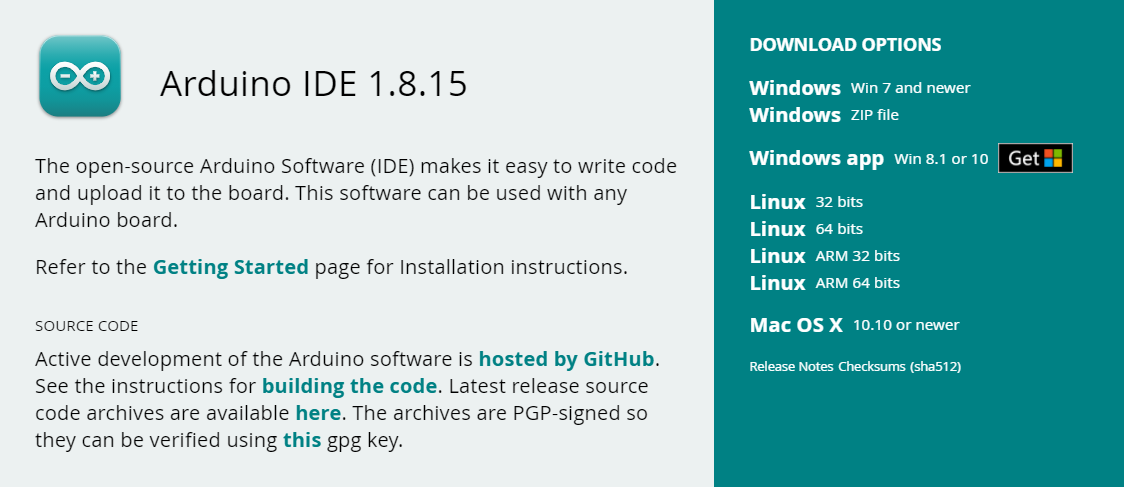
\includegraphics[width=1.0\linewidth]{Nano33BLESense/Installation-1}
%	\caption{Arduino Creat Agent Installation}
%	\label{fig:arduino-creat-agent-installieren}
%\end{figure}




\section{Development}


\subsection{Introduction}

This developer manual is created to help developers to understand the project and to implement their own ideas in to this project after understanding the major aspects of the project.

\subsection{System Requirements}

\fcolorbox{blue}{blue!10}{\begin{minipage}{\textwidth}
    \begin{center}
        \begin{tabular}{llm{90mm}} 
            %\multicolumn{3}{l}{\large \textcolor{blue}{ Tech Specs of Arduino Nano 33 BLE Sense}} \\ \hline
            \\ \textbf{\MapleCommand{\textcolor{blue}{Operating System}}}  & Windows 7 or above, MacOS X or higher \\
            \textbf{\MapleCommand{\textcolor{blue}{CPU}}}  & Intel i3 or above\\
            \textbf{\MapleCommand{\textcolor{blue}{RAM}}}  & Min 2GB\\
            \textbf{\MapleCommand{\textcolor{blue}{Arduino IDE}}}  & V. 1.1819 \\
            \textbf{\MapleCommand{\textcolor{blue}{Boards}}}  & Arduino mBED OS Nano \\
            \textbf{\MapleCommand{\textcolor{blue}{Libraries}}}  & LSM9DS1 \\
            \textbf{\MapleCommand{\textcolor{blue}{Interface}}}  & USB port \\			
        \end{tabular}
    \end{center}
\end{minipage}}

This section describes the system requirements needed for the program to work. 

Since the software is light, the software can be installed on almost all platforms and can be worked up on. 

ARM Cortex M4 Microcontroller (MCU) is present on the Arduino Nano BLE 33 Sense, attached on a stick. 

The software is optimized to run on low power MCU that only runs on 64MHz and 256 kbs of RAM.

A USB cable is required to connect the arduino board to the computer. However,  the wooden stick for the wand is optional. The board orientation plays a major role in prediction of gestures and a change in orientation may result in false positives.



\subsection{Overview of the Program}
This program is designed to detect gestures waved by the user. The model was initially trained with three gestures namely wing , ring and slope where the training data has been stored in to a data set. This program can be further developed by adding more cases for further gestures and adding more cases in the GesturePredictor.cpp file which will be explained in the further sections. 

\section {Code Structure}

The code includes 12 major files. These files are coded to be compatible for the Arduino Platform. 

\subsubsection{Magic\_Wand}
\begin{figure}[h!]
    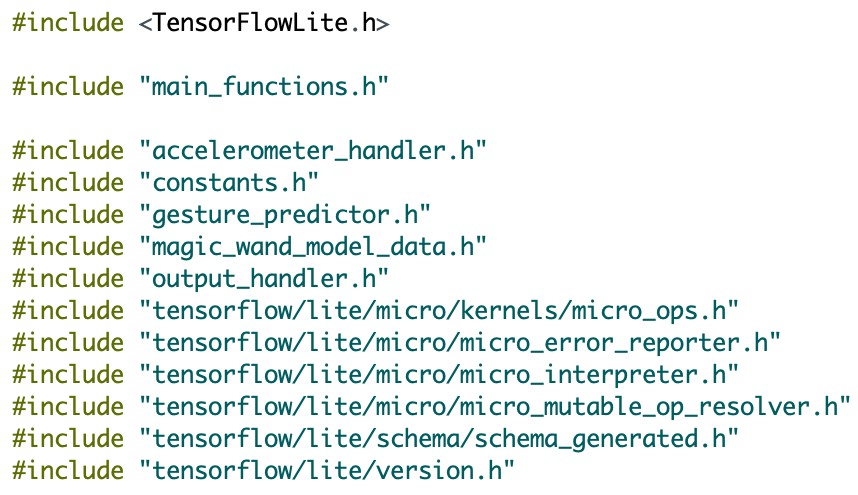
\includegraphics[width=\linewidth]{Nano33BLESense/img12.png}
    \caption{\textbf{Code Snippet function Main header files()}}
    \label{fig:Main()}
\end{figure}


This code snippet \ref{fig:Main()} is the main component file of the program. This file comprises of all the header files and  functions that are used in the program. The program starts by inclusion of all the libraries and header files needed. 




\subsubsection{isMoving()} 

\begin{figure}[h!]
    \includegraphics[width=\linewidth]{Nano33BLESense/ismoving.png}
    \caption{\textbf{Code snippet for isMoving() function }}
    \label{fig:ismoving()}
\end{figure}


Using the function isMoving() shown in \ref{fig:ismoving()} the program checks if the wand is still or moving and returns a boolean value 0 or 1. The isMoving() function works by checking the most recent accelerometer values. 

A constant called "gravity" is intialised and equated to 1000 milli G's. The movement is predicted by subtracting this gravity from the obtained accelerometer values from x,y and z. 

We have inputed a threshold of 40.0f in order to detect any movement. This can be tweaked by the user if the person wants even slightest of the movements to be detected. 

\subsubsection{RecognizeGestures()}

\begin{figure}[h!]
    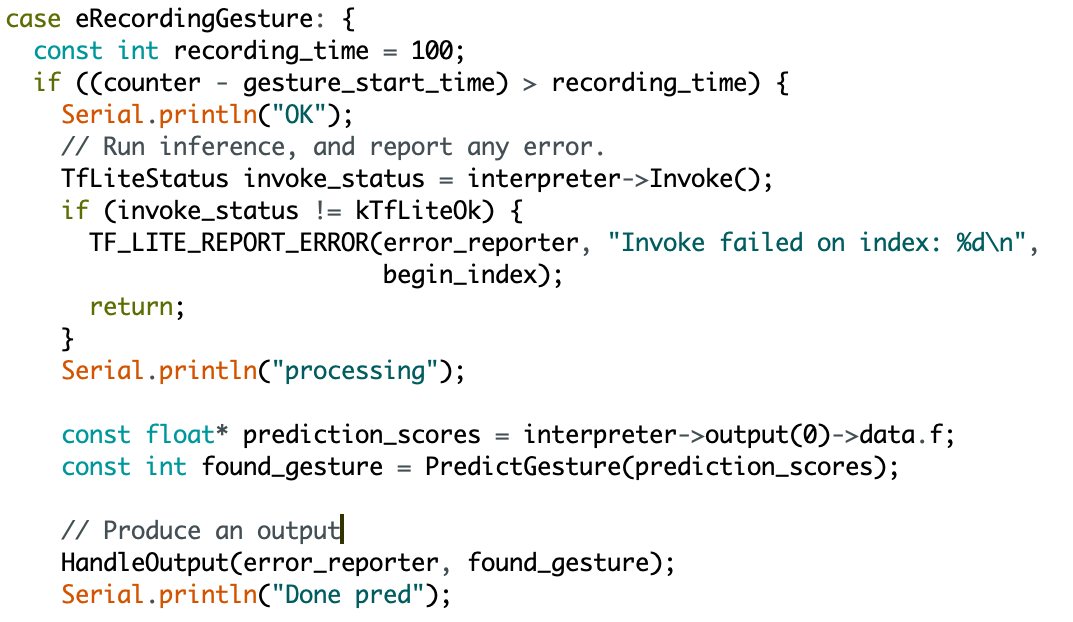
\includegraphics[width=\linewidth]{Nano33BLESense/RecordingGesture.png}
    \caption{\textbf{Code snippet that shows processing of the waved gestures}}
    \label{fig:img14}
\end{figure}

The code snippet shown in \ref{fig:img14} shows a void function and does not return any values. The main objective of this function is to check whether the wand is still or moving. A variable called state is assigned initially and is checked for multiple cases which mentions whether the wand moves or if the wand is kept still. Incase it is moving, the model then records and predicts the gesture.

\subsubsection{Cases - ePendingStillness} 


\begin{figure}[h!]
    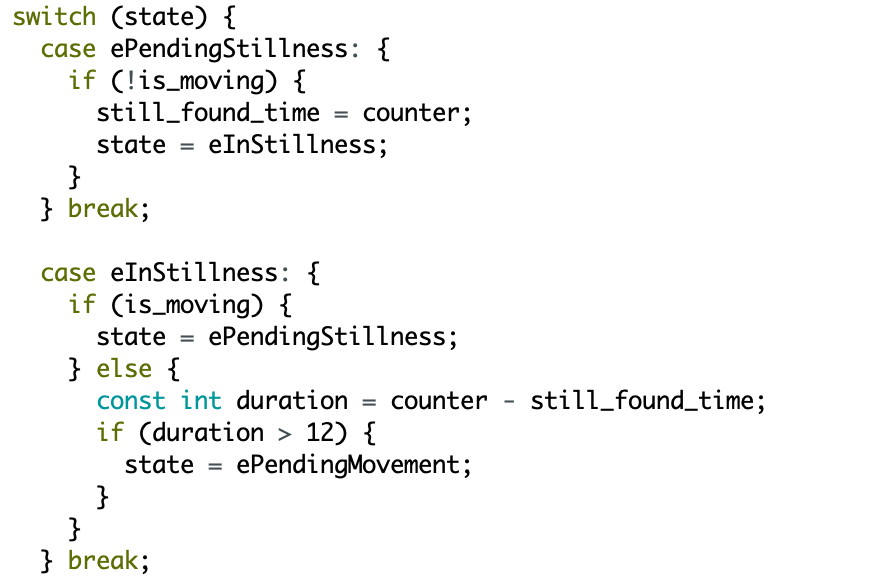
\includegraphics[width=\linewidth]{Nano33BLESense/pending.png}
    \caption{\textbf{The pending switch case that checks if wand is moving or not}}
    \label{pending}
\end{figure}
These switch cases shown in \ref{pending} ensure that the wand is still by utilising the isMoving() function mentioned earlier. A incremental "counter" variable is used at the end of the switch case statement that increments after every iteration. 

\subsubsection{ePendingStillness }
\begin{figure}[h!]
    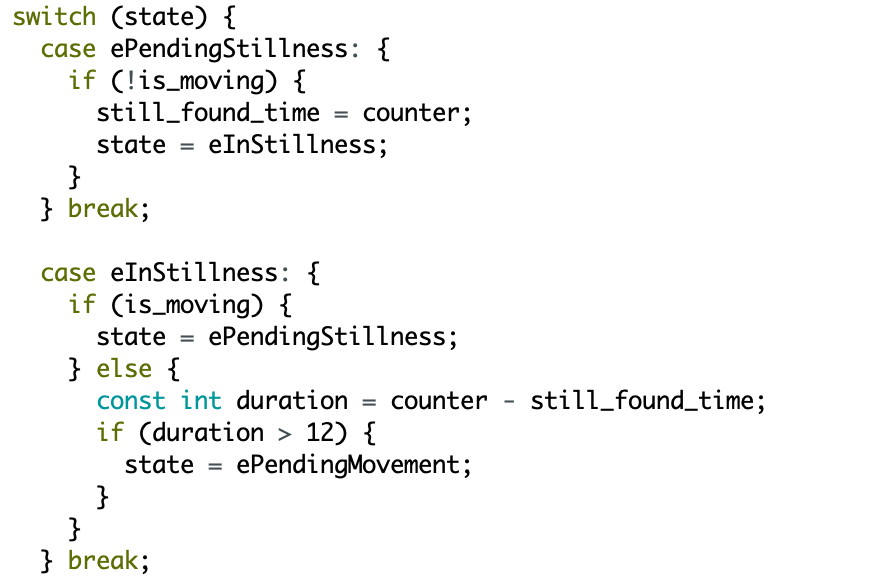
\includegraphics[width=\linewidth]{Nano33BLESense/pending.png}
    \caption{\textbf{Code snippet checking if the wand moves or not}}
    \label{instillness}
\end{figure}
Initially the state is assigned to as ePendingStillness in the code snippet \ref{pending} . The switch case checks if the wand is moving or not. An "if" statement checks if its moving or not and then the value of the counter is equated to a variable "still\_found\_time".The state of the wand is assigned as eInStillness if the "if" condition is satisfied.

\subsubsection{eInStillness} 
\begin{figure}[h!]
    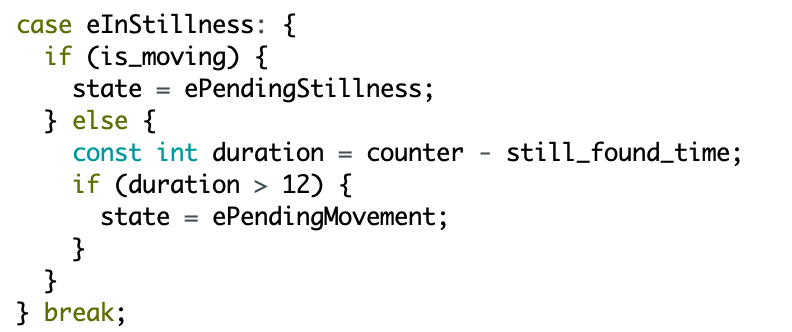
\includegraphics[width=\linewidth]{Nano33BLESense/instillness.png}
    \caption{\textbf{Code snippet to check if the wand is still}}
    \label{instillness}
\end{figure}

An if else statement is used in this case statement as shown in \ref{instillness}. If the boolean value returned from the isMoving() function is true , the "state" is considered as "eInStillness" which means the wand is stationary. If that condition is not satisfied, a new variable "duration" is initialised and calculated by subtracting  the value of "still\_found\_time" from the "counter".
If the calculated duration is greater than 25 which is input by the user, state is assigned as ePendingMovement. This means that the wand is moving and is ready to accept and record gestures from the wand. 
An if statement is used to check the value of the variable "duration", this can be tweaked by the user for lesser values to interpret even the slightest movement. 

\subsection{Cases - ePendingMovement, eRecordingGesture} 

\begin{figure}[h!]
    \includegraphics[width=\linewidth]{Nano33BLESense/pending1.png}
    \caption{\textbf{Code snippet to check if the wand is still}}
    \label{pending1}
\end{figure}


These cases shown in \ref{pending1} form the second part of the switch case statements. These cases makes the computer to accept, record and check the gestures done by the user. 

\textbf{ePendingMovement}

Checks the state of the wand and if the condition is accepted, the command is given to accept new gestures by the output "New Gesture" .


\textbf{eRecordingGesture}

Once the wand starts accepting new gestures, these gestures has to be recorded in order to be checked and compiled.  After waving the gesture, the output window shows "processing" and these values are stored in to Prediction scores and this is  passed in to a  function PredictGesture(). The value obtained earlier is then passed through the function Handle Output() in order to display the gesture waved. The state is then changed back to ePendingStillness and the program continues its iteration.

\textbf{default}

This case is evoked if none of the above cases are satisfied by showing an error. 

\subsubsection{CaptureGestureData()}

\begin{figure}[h!]
    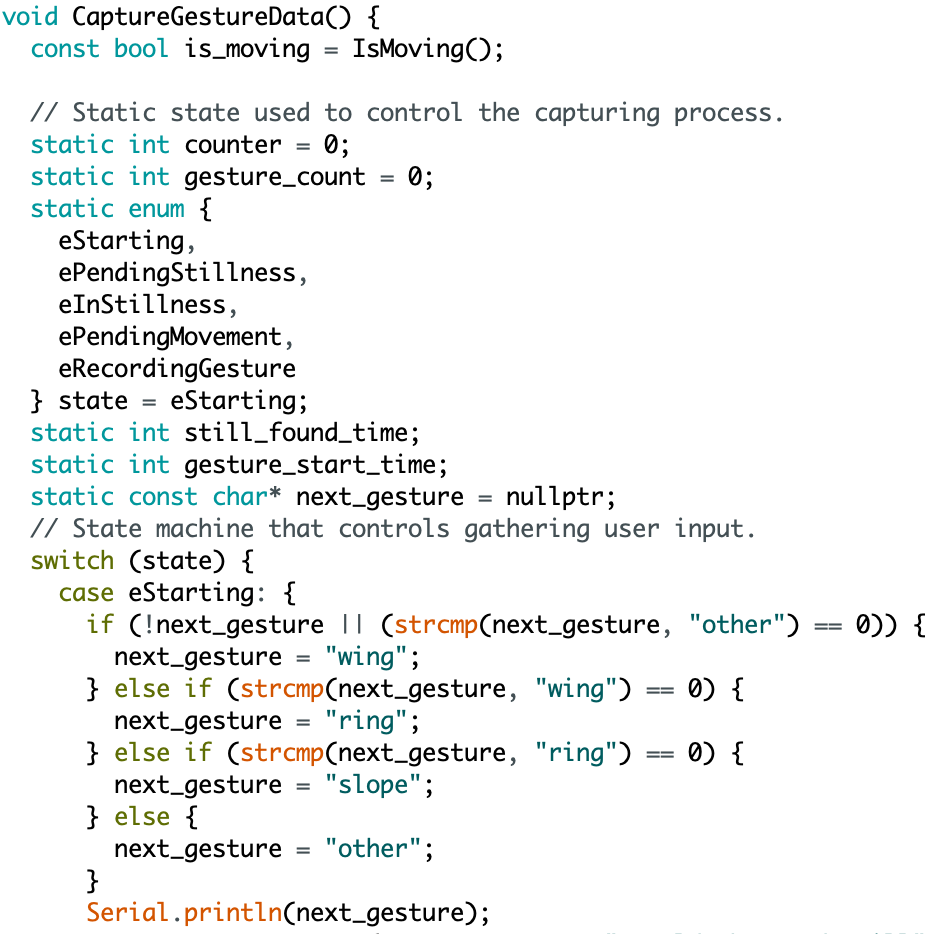
\includegraphics[width=\linewidth]{Nano33BLESense/capture.png}
    \caption{\textbf{Code snippet showing capturing gesture function for training}}
    \label{capture}
\end{figure}

This function shown in \ref{capture} is used for training the magic wand. Different prompts are given to the user to wave a gesture and these data can be fed in to the Python code to gather training data. This ensures that your model is more robust.

The function is similar to the RecognizeGestures()  and has all the switch cases mentioned earlier. The only difference about this function is that it gathers training data and does not predict any gesture or record them.

\subsubsection{loop()} 

\begin{figure}[h!]
    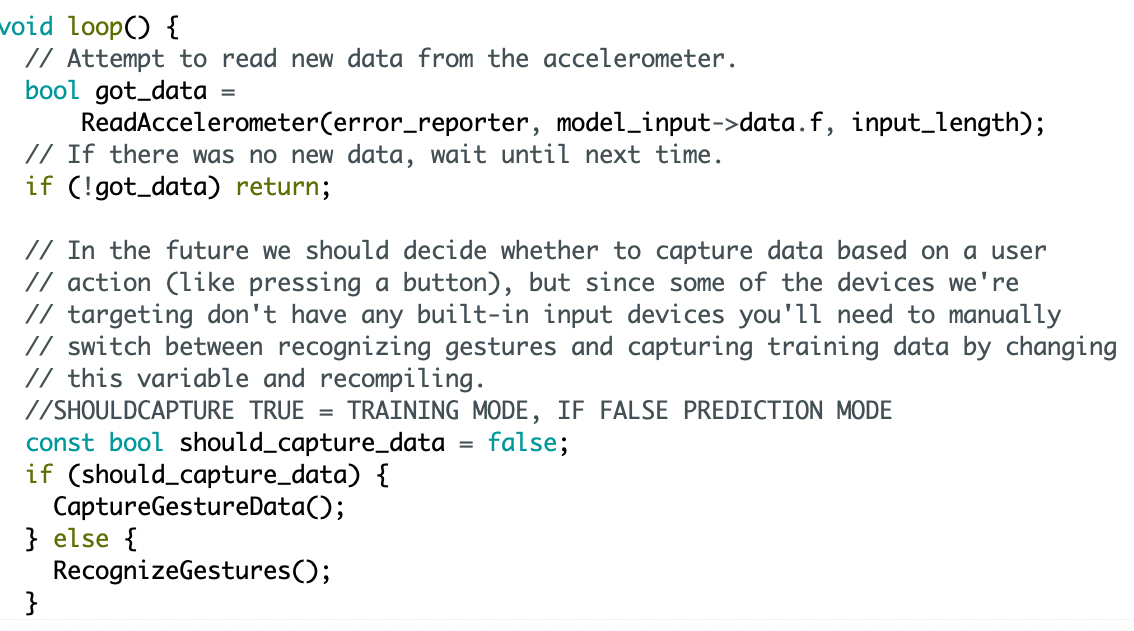
\includegraphics[width=\linewidth]{Nano33BLESense/loop.png}
    \caption{\textbf{Code snippet showing the loop() function in the program}}
    \label{loop}
\end{figure}
This function fragment shown in \ref{loop} attempts to read new acceleroemeter data. A variable named "should\_capture\_data" is initialised and assigned a "false" value. This means that the program is in prediction mode. Changing this value to "true" changes it into training mode and the user can wave gestures, and feed the data to a python notebook to create model data. 

\subsection{arduino\_acceleometer\_handler}

\begin{figure}[h!]
    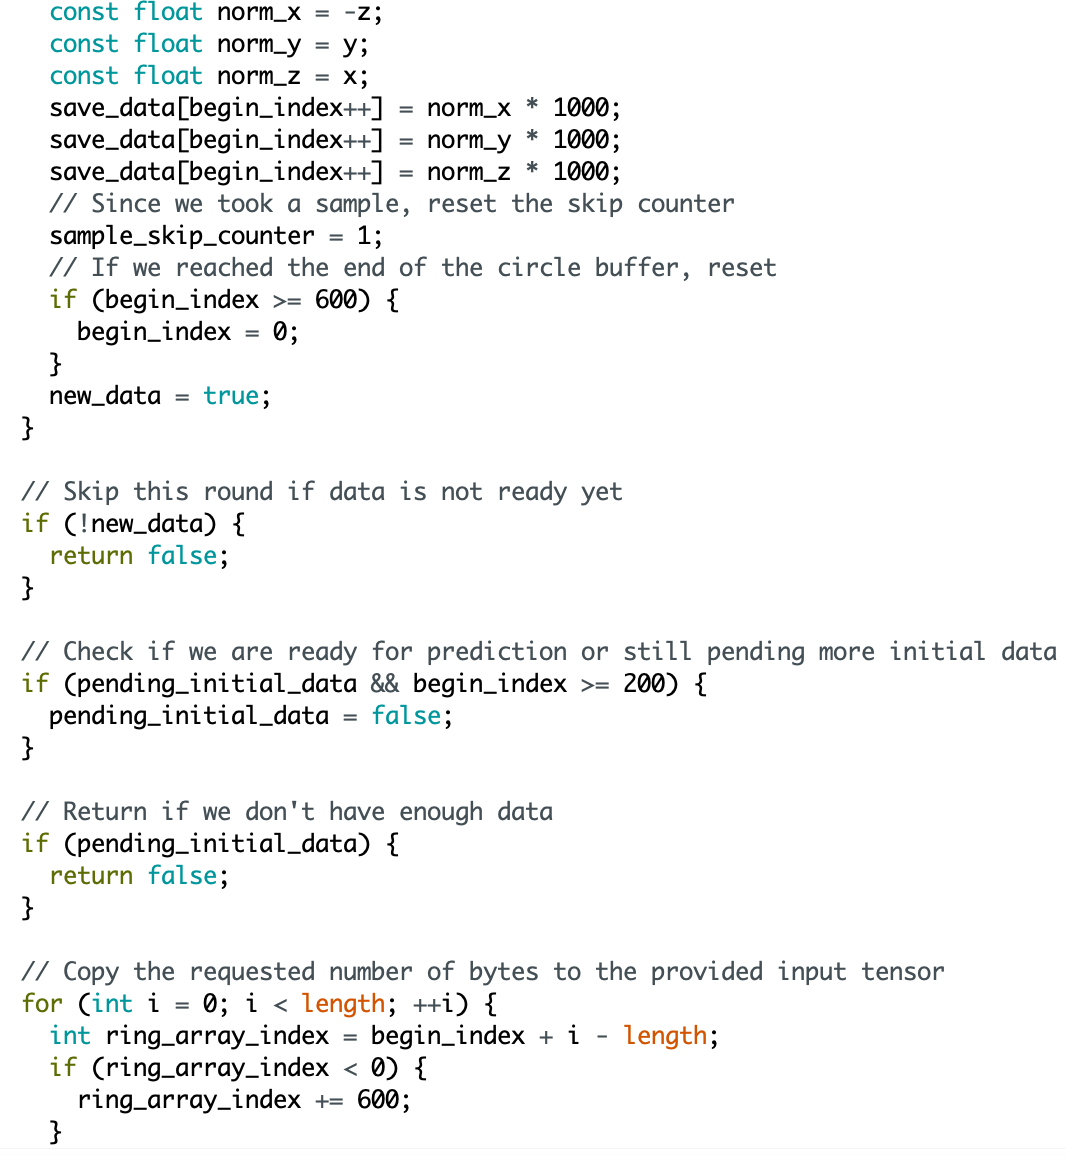
\includegraphics[width=\linewidth]{Nano33BLESense/accel.png}
    \caption{\textbf{The accelerometer handler function}}
    \label{accel}
\end{figure}

The function shown in \ref{accel}  uses input tensor with accelerometer data to calculate the necessary values. 


The value of the accelerometer is recorded in this function when the gesture is waved. Three variables are initialized to store the x, y, and z axis readings. 
These readings are then saved in to an array named "saved\_data" . The array indices for the array is used by the variable "begin\_index" 


These readings are then saved in adjacent array indices with the help of a "++" increment operator. 20 readings per gesture are collected. When the array index crosses 600, the counter resets and a new gesture can be waved. These values can be increased or decreased according to users preferences. 

\subsubsection{gesture\_predictor} 

\begin{figure}[h!]
    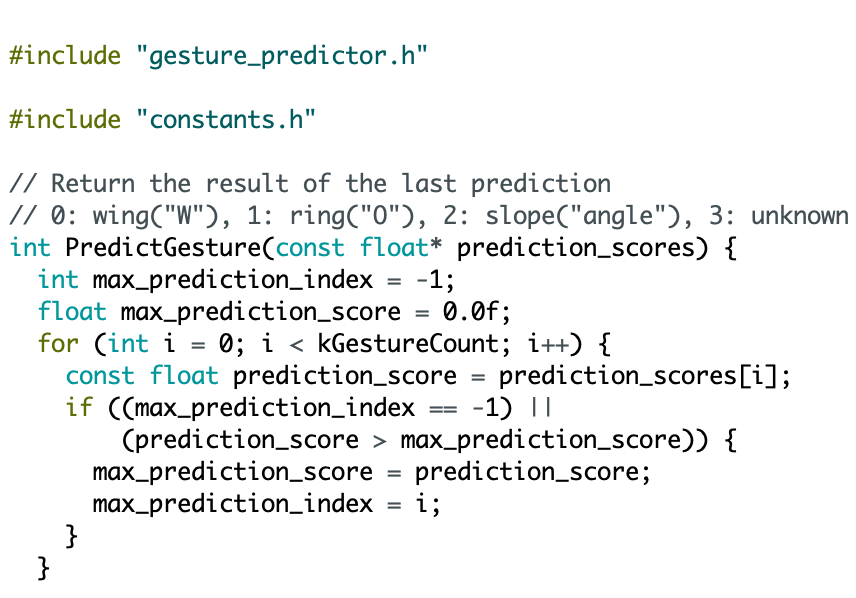
\includegraphics[width=\linewidth]{Nano33BLESense/gest.png}
    \caption{\textbf{Gesture Predictor function}}
    \label{gest}
\end{figure}

The code snippet in \ref{gest} shows the code snippet for gesture predictor.
After the collection of data, the program would be filled with lots of data and has to indicate to us which gesture has been made. Two main things are carried out by this function 

Check whether the gesture probability meets a minimum threshold and also checks if the gesture has been detected over a certain number of inferences. 


This function returns the predicted gesture by returning numeric values 0,1, 2 and 3 for Wing, Ring, Slope and unknown respectively. 
Initially the "prediction scores" obtained from the main is passed on to the function in which a "maxPredictionScore" and "maxPrediction Index".
These values  above are then compared to "kNoGesture" and "kDetectionThrehsold", then the value of found gesture variable is found which is equal to max prediction index. 



\subsection{Arduino\_Output\_Handler} 

\begin{figure}[h!]
    \includegraphics[width=\linewidth]{Nano33BLESense/handleoutput.png}
    \caption{\textbf{The code handling the output}}
    \label{op}
\end{figure}

The function shown in \ref{op}  output handler is to display the output according to the value it receives from the PredictGesture() function. It simply displays the gesture waved, which in this case is Wing, Ring and Slope. 

\subsection{main\_functions} 

\begin{figure}[h!]
    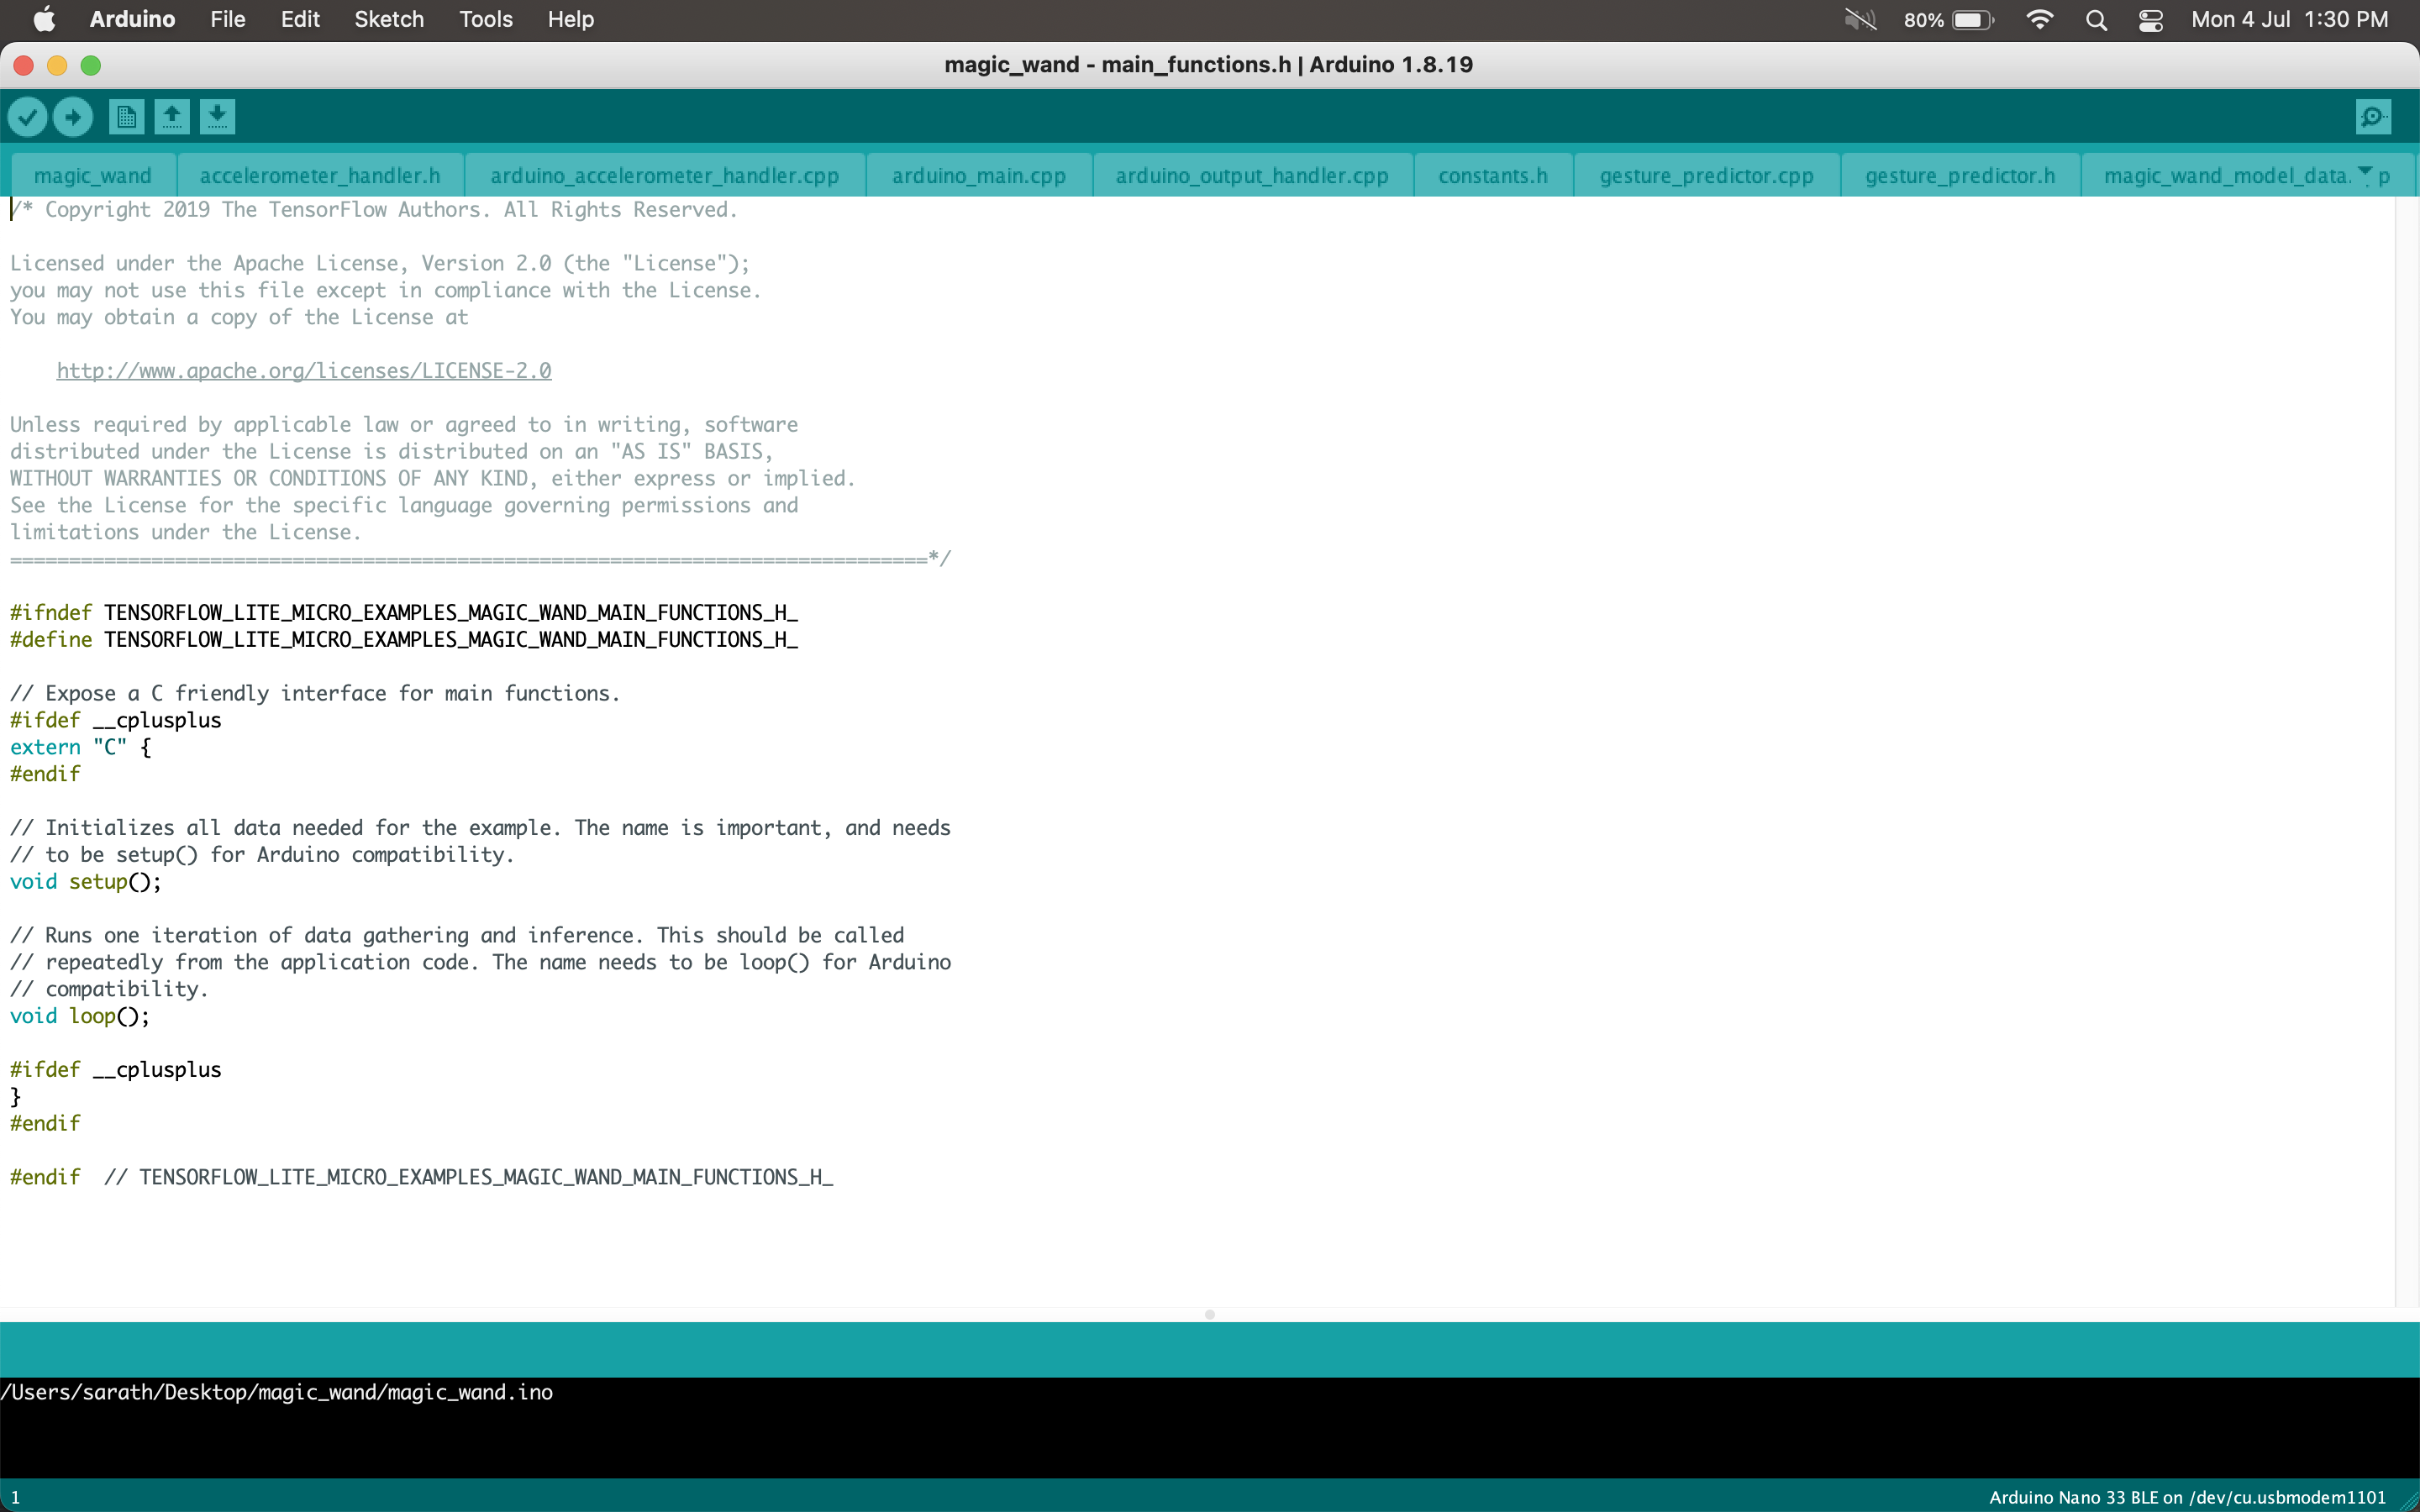
\includegraphics[width=\linewidth]{Nano33BLESense/mainf.png}
    \caption{\textbf{Code snippet showing the loop() function in the program}}
    \label{mainf}
\end{figure}
The code snippet shown in \ref{mainf} contains two functions, setup() and loop(). The setup() function intialises all the necessary values required for the program to function. The loop() function runs once and iterates the data to predict the gesture. 

\subsection{constants.h}


\begin{figure}[h!]
    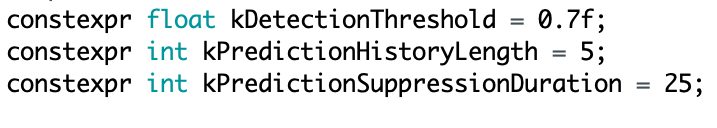
\includegraphics[width=\linewidth]{Nano33BLESense/constexpr.png}
    \caption{\textbf{Code displaying threshold values}}
    \label{constexpr}
\end{figure}

This code snippet shown in \ref{constexpr} contains the expected accelerometer data frequency. A numerical value is assigned to the gestures, Wing, Ring, Slope and unknown as 0,1,2 and 3 respectively. A 'kDetectionthreshold" variable is present which can be tweaked to ensure the quality of results or outputs obtained. Higher values of the variable means that the gesture wave should be more accurate to the training data.


\subsection{Magic Wand Program Workflow}



\tikzstyle{decision} = [diamond, draw, fill=white, 
text width=5.5em, text badly centered, node distance=3cm, inner sep=0pt]
\tikzstyle{block} = [rectangle, draw, fill=blue!20, 
text width=9em, text centered, rounded corners, minimum height=2.5em]
\tikzstyle{line} = [draw, -latex']
\tikzstyle{cloud} = [draw, ellipse,fill=white, node distance=2cm,
minimum height=2em]

\begin{center}
    \centering
    \begin{tikzpicture}[node distance = 2.2cm, auto]
        
        \node [cloud,fill=green!50,node distance=1cm] (init) {Start};
        \node [block, below of=init] (start) {Waiting for movement};
        \node [decision,fill=yellow!20,below of=start] (select) {Check if moving};
        \node [block, left of=select,node distance=5cm] (invalid){Wand is still in stillness};
        %		\node [block, below of=select,node distance=3cm] (neighbour) {Pending movement};
        \node [block, below of=select, node distance=3cm] (distance) {Record gesture};
        \node [block, below of=distance,node distance=2cm] (update) {Gesture Predictor};
        \node [block, below of=update,node distance=2cm] (run) {Check the predicted score};
        \node [decision,fill=yellow!20,below of=run, node distance=3cm] (decide) {Gesture found?};
        \node [cloud,fill=red!50, left of=decide,node distance=5cm] (none){"Unkown"};
        \node [block, below of=decide, node distance=3cm] (stop) {Display Output};
        \node [cloud,fill=red!50, below of=stop,node distance=2cm] (end) {End};
        \path [line] (init) -- (start);
        \path [line] (start) -- (select);
        \path [line] (select) --node {Yes} (distance);
        \path [line] (select) -- node[near start]{No}  (invalid);
        \path [line] (invalid) |-  (start);
        %	\path [line] (neighbour) -- (distance);
        \path [line] (distance) -- (update);
        \path [line] (update) -- (run);
        \path [line] (run) -- (decide);
        \path [line] (decide) -- node {Yes}(stop);
        \path [line] (decide) -- node[near start]{No}  (none);
        \path [line] (stop) -- (end);
        %	\path [line] (solution) -- (stop);
        
    \end{tikzpicture}
    \captionof{figure}{Magic Wand Program Workflow}
\end{center}


%%%%%%%%%%%%%%%%%%%%%


\section{FAQs} 

\begin{enumerate}
    
    \item Why LEDs are not blinking?
    
    A. Check the connection, also confirm the program is uploaded properly without any errors.
    
    \item Why does the orange light blink sometimes?
    
    A. It is a programmable LED and in this case it blinks when a process is running.
    
    \item What is the button present on the board?
    
    A. It is the reset button, which you can use for resetting the program. 
    
    \item How to reset the magic wand?
    
    A. Press the reset button present on the board. 
    
    \item How should I hold the magic wand?
    
    A. Hold the magic wand according to how it was trained. However handle with care by not harming the components and sensors present on the board.
    
    \item Why I am not getting the gesture which I waved?
    
    A. Hold the wand in a manner how you trained it, also train it with more datasets.
    
    \item Is it water and fire resistant?
    
    A. No, it not. keep away from water or fire.
    
    \item What is input voltage required for the magic wand?
    
    A. Arduino Nano 33 BLE only supports 3.3V.So make sure you do not connect it to any other input signals to this board or else it will be damaged. 
    
    \item Is it wireless, Can I connect it with Bluetooth?
    
    A. It can be connected with the Bluetooth, but as there is no inbuilt battery it should be powered by connecting it with the Micro-B USB cable to the computer.
    
    \item How to turn on/turn off the magic wand?
    
    A. The board can be powered via USB connector. Once turned on, Power LED lights up.
    
\end{enumerate}

